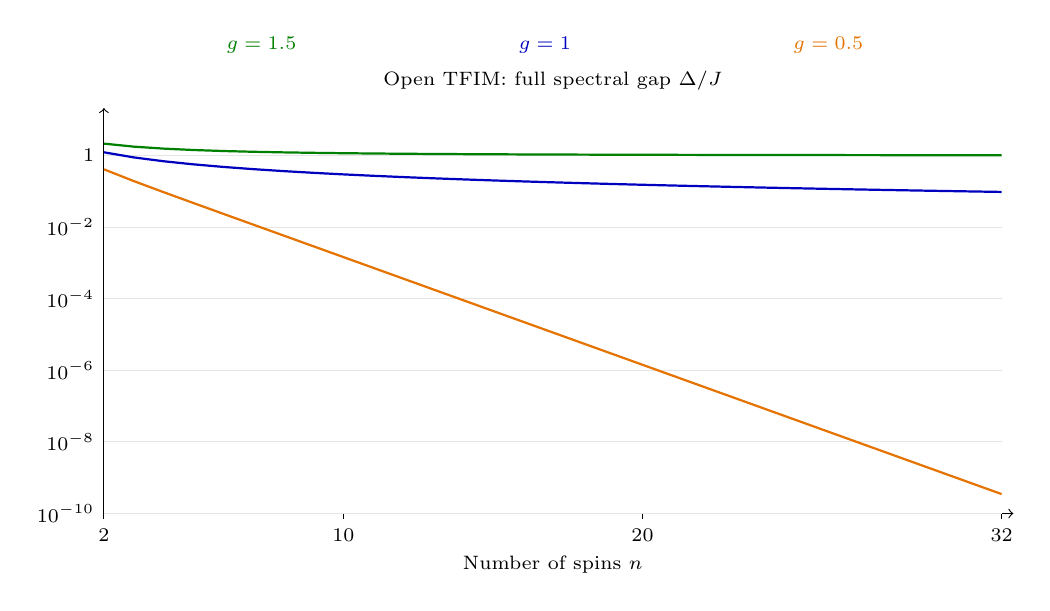
\begin{tikzpicture}[x=1cm,y=1cm,font=\scriptsize]
\draw[->] (0.0000,0.0000)--(11.5500,0.0000);
\draw[->] (0.0000,0.0000)--(0.0000,5.1500);
\draw (0.0000,0.0000)--+(0,-.07) node[below] {$2$};
\draw (3.0400,0.0000)--+(0,-.07) node[below] {$10$};
\draw (6.8400,0.0000)--+(0,-.07) node[below] {$20$};
\draw (11.4000,0.0000)--+(0,-.07) node[below] {$32$};
\draw[gray!20] (0.0000,0.0000)--+(11.4000,0);
\node[left] at (0.0000,0.0000) {$10^{-10}$};
\draw[gray!20] (0.0000,0.9091)--+(11.4000,0);
\node[left] at (0.0000,0.9091) {$10^{-8}$};
\draw[gray!20] (0.0000,1.8182)--+(11.4000,0);
\node[left] at (0.0000,1.8182) {$10^{-6}$};
\draw[gray!20] (0.0000,2.7273)--+(11.4000,0);
\node[left] at (0.0000,2.7273) {$10^{-4}$};
\draw[gray!20] (0.0000,3.6364)--+(11.4000,0);
\node[left] at (0.0000,3.6364) {$10^{-2}$};
\draw[gray!20] (0.0000,4.5455)--+(11.4000,0);
\node[left] at (0.0000,4.5455) {$1$};
\node at (5.7000,-0.6500) {\lr{Number of spins} $n$};
\node at (5.7000,5.5000) {\lr{Open TFIM: full spectral gap} $\Delta/J$};
\draw[green!50!black,thick,] plot coordinates {(0.00000,4.69769) (0.38000,4.65924) (0.76000,4.63405) (1.14000,4.61647) (1.52000,4.60366) (1.90000,4.59402) (2.28000,4.58657) (2.66000,4.58069) (3.04000,4.57598) (3.42000,4.57214) (3.80000,4.56898) (4.18000,4.56634) (4.56000,4.56411) (4.94000,4.56222) (5.32000,4.56060) (5.70000,4.55920) (6.08000,4.55799) (6.46000,4.55692) (6.84000,4.55599) (7.22000,4.55516) (7.60000,4.55443) (7.98000,4.55378) (8.36000,4.55319) (8.74000,4.55266) (9.12000,4.55219) (9.50000,4.55176) (9.88000,4.55137) (10.26000,4.55102) (10.64000,4.55069) (11.02000,4.55039) (11.40000,4.55012)};
\node[text=green!50!black] at (2.00,5.95) {$g=1.5$};
\draw[blue!75!black,thick,] plot coordinates {(0.00000,4.58729) (0.38000,4.52247) (0.76000,4.47351) (1.14000,4.43423) (1.52000,4.40145) (1.90000,4.37332) (2.28000,4.34869) (2.66000,4.32679) (3.04000,4.30707) (3.42000,4.28914) (3.80000,4.27271) (4.18000,4.25753) (4.56000,4.24344) (4.94000,4.23029) (5.32000,4.21796) (5.70000,4.20635) (6.08000,4.19539) (6.46000,4.18500) (6.84000,4.17513) (7.22000,4.16573) (7.60000,4.15676) (7.98000,4.14818) (8.36000,4.13996) (8.74000,4.13206) (9.12000,4.12447) (9.50000,4.11716) (9.88000,4.11011) (10.26000,4.10331) (10.64000,4.09673) (11.02000,4.09036) (11.40000,4.08419)};
\node[text=blue!75!black] at (5.60,5.95) {$g=1$};
\draw[orange!90!black,thick,] plot coordinates {(0.00000,4.37147) (0.38000,4.22166) (0.76000,4.08034) (1.14000,3.94202) (1.52000,3.80471) (1.90000,3.66773) (2.28000,3.53086) (2.66000,3.39401) (3.04000,3.25718) (3.42000,3.12035) (3.80000,2.98351) (4.18000,2.84668) (4.56000,2.70985) (4.94000,2.57302) (5.32000,2.43619) (5.70000,2.29936) (6.08000,2.16252) (6.46000,2.02569) (6.84000,1.88886) (7.22000,1.75203) (7.60000,1.61520) (7.98000,1.47836) (8.36000,1.34153) (8.74000,1.20470) (9.12000,1.06787) (9.50000,0.93104) (9.88000,0.79421) (10.26000,0.65737) (10.64000,0.52054) (11.02000,0.38371) (11.40000,0.24688)};
\node[text=orange!90!black] at (9.20,5.95) {$g=0.5$};
\end{tikzpicture}